\documentclass[12pt]{article}
\usepackage[utf8]{inputenc}
\usepackage[spanish]{babel}
\usepackage{textcomp}
\usepackage{graphicx}

\usepackage{geometry}
\usepackage{colortbl}
\usepackage{array}
\usepackage{float}
\usepackage{enumitem}
\usepackage[
    backend=biber,
    style=phys,
    sorting=none,
    giveninits=true,
    articletitle=false,        % Sin títulos de artículos
    biblabel=brackets,
    chaptertitle=false,
    pageranges=false
]{biblatex}


\addbibresource{referencias.bib}
\usepackage{amsmath,amssymb}
\geometry{left=2.5cm, right=2.5cm, top=2.5cm, bottom=2.5cm}
\usepackage{titlesec}
\newcommand{\mcL}{\mathcal{L}}
\newcommand{\mcH}{\mathcal{H}}
\newcommand{\mcS}{\mathcal{S}}
\newcommand{\mcM}{\mathcal{M}}
\newcommand{\ket}[1]{\lvert #1 \rangle}
\newcommand{\bra}[1]{\langle #1 \rvert}
\newcommand{\braket}[2]{\langle #1 | #2 \rangle}


% Estilo para títulos de sección
\titleformat{\section}{\normalfont\Large\bfseries}{\thesection}{1em}{}
\usepackage{atbegshi}
\spanishdecimal{.}
\begin{document}

% Portada estilizada

    \begin{center}
    
        % Logos e institución
        
\includegraphics[width=4cm]{logos/uaem.png} \hfill
        
\includegraphics[width=5cm]{logos/ciicap.png} \\[2cm]
        
        % Línea separadora superior
        \hrulefill \\[0.4cm]

        % Programa educativo
        {\Large \textsc{Maestría en Ingeniería y Ciencias Aplicadas}} \\[0.5cm]

        % Título del reporte
        \hrulefill \\[0.4cm]
        {\LARGE \textbf{Fluorescencia Resonante Intermitente con Ecuaciones Estocásticas de Schrodinger}} \\[0.4cm]
        \hrulefill \\[0.5cm]

        % Subtítulo y periodo
        {\Large \textbf{Cuarto Reporte Semestral}} \\[0.2cm]
        {\large \textbf{Periodo: Enero - Agosto 2026}} \\[2cm]
        
        \vfill

        % Información del estudiante
        \textbf{Alumno:} \\[0.2cm]
        {\Large L. T. Kevin Martínez Franco} \\[1.5cm]

        % Información del asesor
        \textbf{Asesor:} \\[0.2cm]
        {\Large Dr. Héctor Manuel Castro Beltrán} \\[2cm]

        % Fecha
        {\large \textbf{\today}} \\[2cm]
        
        % Línea final
        \hrulefill

    \end{center}


% Resumen
\section{Resumen}

Durante el semestre se lograron avances significativos en el estudio de la fluorescencia resonante intermitente, obteniendo resultados novedosos en varios frentes. En primer lugar, se completó la detección homodina balanceada; habíamos obtenido que en las cuadraturas en $\pi/2$ y $0$ se identifican, respectivamente, el pico angosto con laterales y el pico central coherente, y el nuevo resultado es que la combinación de estas cuadraturas reconstruye el espectro completo de fluorescencia con la forma del triplete de Mollow. En tercer lugar, se desarrolló un análisis de la fluorescencia intermitente con bombeo incoherente, tanto mediante la ecuación maestra como con trayectorias de saltos. De este estudio se obtuvieron distribuciones que evidencian la alternancia entre periodos brillantes y oscuros, con diferencias notables respecto al átomo de tres niveles con dinámica coherente por excitación láser que se estudió en semestres anteriores. Las nuevas predicciones teóricas se confirmaron mediante simulaciones tanto en promedios como en momentos.

En conjunto, estos avances fortalecen el enfoque general de la tesis, permitiendo pulir los detalles del análisis espectral de la fluorescencia resonante intermitente y extender los resultados a un nuevo sistema de tres niveles con bombeo incoherente, lo cual abre nuevas líneas de investigación para el futuro próximo.


% Introducción
\section{Introducción}
La disipación, entendida como la pérdida irreversible de energía y coherencia de un microsistema, surge del acoplamiento a un macrosistema o reservorio con un número de grados de libertad extraordinariamente grande. En la práctica, resulta imposible resolver la dinámica completa mediante la ecuación de Schrödinger para el sistema total, ya que el espacio de Hilbert del reservorio es inaccesible desde un punto de vista computacional y experimental. Esta imposibilidad obliga a recurrir a descripciones efectivas, donde el efecto del entorno se incorpora a través de operadores de disipación en la ecuación maestra o mediante trayectorias estocásticas, como en el formalismo de Monte Carlo de saltos cuánticos.
\begin{figure}[H]
    \centering
    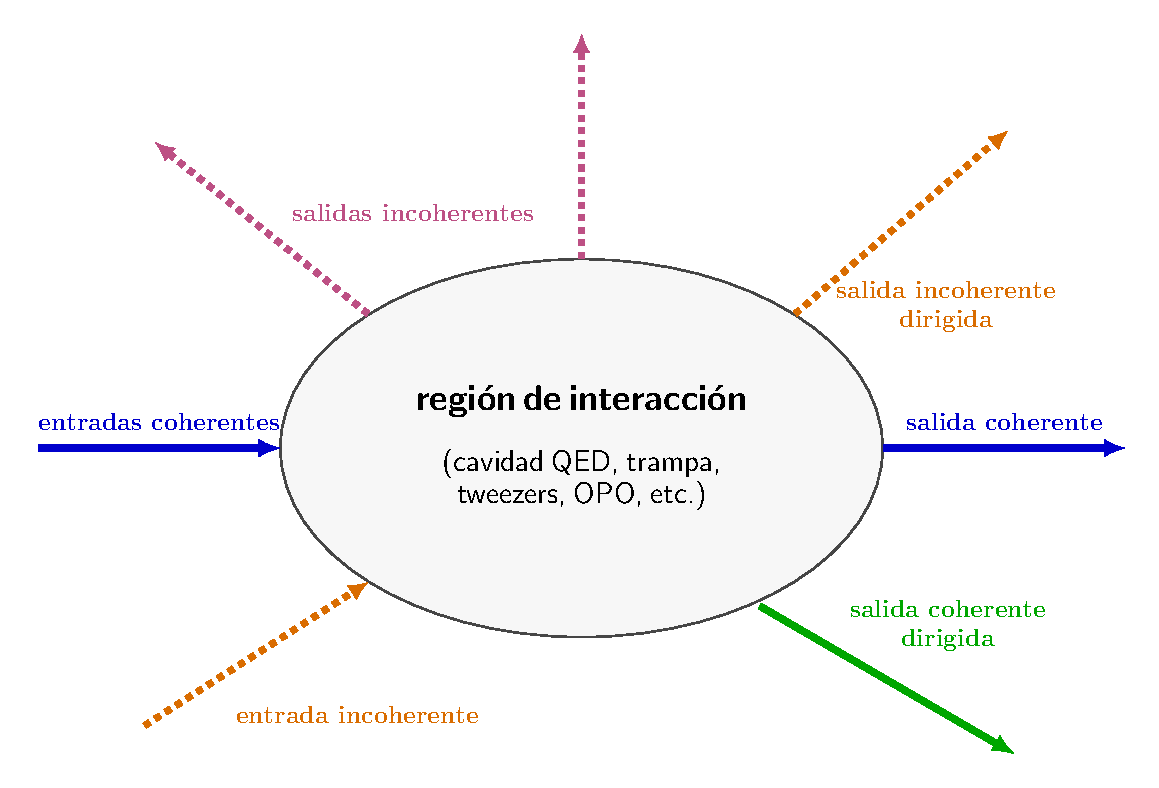
\includegraphics[width=0.8\textwidth]{imagenes/SQA.pdf}
    \caption{Esquema de un sistema cuántico abierto, donde el sistema de interés (en azul) interactúa con un entorno (en gris) que induce procesos de disipación y decoherencia.}
    \label{fig:region_interaccion}
\end{figure}
En la Figura~\ref{fig:region_interaccion} se ilustra el esquema general de los sistemas estudiados en este proyecto. La región de interacción que puede corresponder a una cavidad QED, una trampa de iones, pinzas ópticas (tweezers), un OPO u otros dispositivos constituye el núcleo del sistema cuántico abierto. Dicha región recibe entradas tanto coherentes (como campos láser) como incoherentes (como bombeo estocástico o ruido), y genera salidas que pueden ser igualmente coherentes o incoherentes, dependiendo del régimen de operación. El análisis de estas señales de salida ya sea en su componente coherente dirigida o en su emisión incoherente permite extraer información sobre la dinámica interna del sistema, así como caracterizar fenómenos como la fluorescencia resonante, la emisión espontánea dirigida y los efectos de correlación cuántica.

En el caso particular de este proyecto, nos enfocamos en la fluorescencia atómica, donde la región de interacción es un átomo de pocos niveles (dos o tres) iluminado por un campo láser coherente y, en algunos casos, sometido a bombeo incoherente. La salida incoherente emitida por el átomo la fluorescencia propiamente dicha contiene información clave sobre la dinámica de población y coherencias, y su espectro presenta estructuras características como el pico de Mollow o el pico central coherente. Además, mediante técnicas de detección homodina y heterodina balanceada, es posible aislar las contribuciones coherentes e incoherentes, lo que permite reconstruir el espectro completo y estudiar fenómenos como la fluorescencia intermitente, donde el átomo alterna entre periodos brillantes y oscuros debido a la presencia de estados metaestables.

\subsection{Fluorescencia Resonante Intermitente}
La fluorescencia resonante intermitente es el fenómeno en el que la emisión de un sistema cuántico alterna aleatoriamente entre períodos brillantes y oscuros. Esta intermitencia puede originarse por distintos mecanismos físicos dependiendo del sistema considerado.

En este trabajo estudiaremos el caso de un átomo de tres niveles, donde la intermitencia surge mediante el mecanismo conocido como electron shelving, donde el átomo puede quedar atrapado en un estado de larga vida media al que llamamos estado mestable , lo que da lugar a periodos oscuros, mientras que la transición entre los estados de emisión conduce a periodos brillantes.

Para explicar este mecanismo primero describiremos el sistema de tres niveles interactuando con el láser. El láser acopla resonantemente la transición entre el estado base $\ket{g}$ y el estado excitado $\ket{e}$, con frecuencia de Rabi $\Omega$, como se ilustra en la Figura~\ref{fig:3niveles}. El estado excitado puede decaer espontáneamente al estado base con tasa $\gamma$, produciendo los fotones de fluorescencia que observamos experimentalmente. Además, el átomo posee un tercer nivel $\ket{a}$, que se encuentra débilmente acoplado al ciclo principal de excitación y emisión. Trabajaremos en el régimen $\gamma \gg \gamma_d, \gamma_a$, donde la dinámica entre $\ket{g}$ y $\ket{e}$ ocurre mucho más rápido que las transiciones asociadas al tercer nivel.

Cabe mencionar que la tasa ($\gamma_a$) utilizada en este trabajo debe interpretarse como una tasa efectiva. En sistemas atómicos reales, la vida media del estado metaestable puede ser tan larga que la observación numérica y experimental de un número significativo de transiciones requeriría tiempos prohibitivamente grandes. Por esta razón, es común introducir un cuarto nivel auxiliar acoplado ópticamente al estado metaestable, el cual decae rápidamente al estado base. En estas condiciones, la dinámica puede describirse mediante un modelo efectivo de tres niveles caracterizado por una tasa de desexcitación ($\gamma_a$) ajustable.\cite{NaSD86,SNBT86,BHIW86,Carm93}.

\begin{figure}[H]
    \centering
    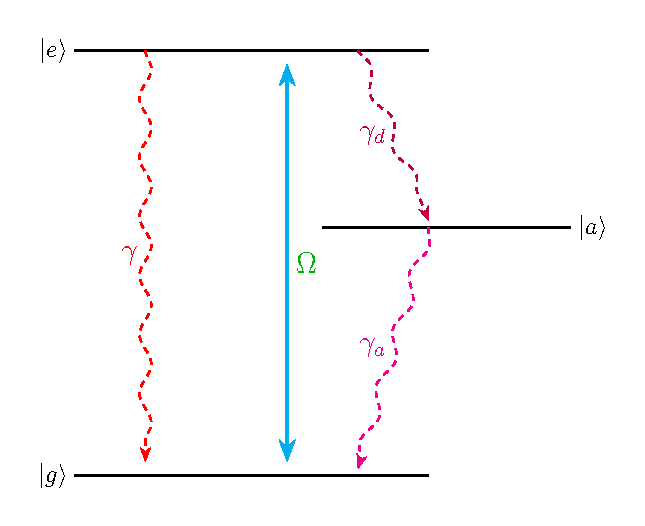
\includegraphics[width=0.7\textwidth]{imagenes/3LA.pdf}
    \caption{Esquema de niveles atómicos con acoplamiento láser representado por $\Omega$ y decaimientos radiativos.}
    \label{fig:3niveles}
\end{figure}
Para completar la descripción del sistema es necesario especificar el Hamiltoniano que describe la interacción coherente entre el átomo y el campo láser. En el marco rotante asociado a la frecuencia del láser, el Hamiltoniano efectivo puede escribirse como

\begin{equation}
\mathcal{H} = \Delta \, \sigma_{eg} \sigma_{ge}
+\frac{\Omega}{2} ( \sigma_{eg} + \sigma_{ge} ) .
\end{equation}
\\
donde

\begin{equation}
\Omega=\frac{\mathbf{d}_{eg}\cdot\mathbf{E}_0}{\hbar}
\end{equation}

es la frecuencia de Rabi asociada al acoplamiento entre el momento dipolar atómico $\mathbf{d}_{eg}$ y la amplitud del campo eléctrico del láser $\mathbf{E}_0$, mientras que

\begin{equation}
\Delta=\omega_{eg}-\nu
\end{equation}

es la desintonía entre la frecuencia de transición atómica $\omega_{eg}$ y la frecuencia del láser $\nu$.


\subsection{Soluciones con ecuacion maestra}
Para resolver la dinámica de este sistema, recurrimos primero a la ecuación maestra bajo las aproximaciones de Born y Markov. La aproximación de Born supone un acoplamiento débil con el entorno, de modo que este permanece inalterado, mientras que la aproximación de Markov desprecia los efectos de memoria del entorno al considerar que su tiempo de correlación es mucho más corto que la dinámica atómica. Con estas consideraciones, la ecuación maestra en forma de Lindblad para nuestro sistema es

\begin{equation}
\dot{\rho} = -\frac{i}{\hbar}[H, \rho] + \sum_k \left( L_k \rho L_k^\dagger - \frac{1}{2}\{L_k^\dagger L_k, \rho\} \right),
\end{equation}


La dinámica del sistema se describe mediante una ecuación maestra markoviana en el marco rotante y bajo la aproximación de onda rotante:

\begin{equation}
\begin{split}
\dot{\rho} ={}& -i\Delta [\sigma_{ee},\rho]
- i\frac{\Omega}{2}[\sigma_{eg}+\sigma_{ge},\rho] \\
&+ \frac{\gamma}{2}\bigl(2\sigma_{ge}\rho \sigma_{eg} - \sigma_{ee}\rho - \rho \sigma_{ee}\bigr) \\
&+ \frac{\gamma_d}{2}\bigl(2\sigma_{ae}\rho \sigma_{ea} - \sigma_{ee}\rho - \rho \sigma_{ee}\bigr) \\
&+ \frac{\gamma_a}{2}\bigl(2\sigma_{ga}\rho \sigma_{ag} - \sigma_{aa}\rho - \rho \sigma_{aa}\bigr).
\end{split}
\end{equation}

Estas ecuaciones están escritas en un marco de referencia que rota a la frecuencia del láser, lo cual elimina las oscilaciones rápidas asociadas al campo externo y permite describir únicamente la dinámica relevante del sistema.

A partir de la ecuación maestra obtenemos el siguiente sistema de ecuaciones diferenciales para las poblaciones y coherencias del sistema:

\begin{eqnarray} 	\label{eq:dotrho_jk}
\dot{\rho}_{eg} &=& i\frac{\Omega}{2} (\rho_{ee} -\rho_{gg})
 -\left( \frac{\gamma_+}{2}  +i\Delta \right) \rho_{eg} \,, \\
%
\dot{\rho}_{ge} &=& -i\frac{\Omega}{2} (\rho_{ee} -\rho_{gg})
 -\left( \frac{\gamma_+}{2}  -i\Delta \right) \rho_{ge} \,,
 	\nonumber 	\\
%
\dot{\rho}_{ee} &=& -i\frac{\Omega}{2} (\rho_{ge} -\rho_{eg})
 	-\gamma_+ \rho_{ee} \,,	\nonumber 	\\
%
\dot{\rho}_{gg} &=& i\frac{\Omega}{2} (\rho_{ge} -\rho_{eg})
	+\gamma_- \rho_{ee} -\gamma_a \rho_{gg}
	+\gamma_a \,.	 	\nonumber
\end{eqnarray}

donde

\begin{eqnarray}
\gamma_+ &=& \gamma + \gamma_d \,, \qquad
\gamma_- = \gamma - \gamma_a \,.
\end{eqnarray}

La ecuación para la población del estado metaestable,

\begin{equation}
\dot{\rho}_{aa} = \gamma_d \rho_{ee} - \gamma_a \rho_{aa},
\end{equation}

ha sido eliminada utilizando la condición de conservación de la probabilidad,
\begin{equation}
\rho_{gg}+\rho_{ee}+\rho_{aa}=1.
\end{equation}

De esta forma, la población del estado metaestable puede expresarse como

\begin{equation}
\rho_{aa}=1-\rho_{gg}-\rho_{ee},
\end{equation}

y sustituirse en la ecuación para $\dot{\rho}_{gg}$,

\begin{equation}
\dot{\rho}_{gg}
=
i\frac{\Omega}{2}(\rho_{ge}-\rho_{eg})
+\gamma\rho_{ee}
+\gamma_a\rho_{aa},
\end{equation}

Obteniéndose de esta manera un sistema reducido de cuatro ecuaciones diferenciales independientes.

La resolución numérica de este sistema se realizó mediante la biblioteca **QuTiP** de Python, lo que permitió obtener la evolución temporal de las poblaciones y coherencias del sistema. Los resultados se muestran en la Figura~\ref{fig:3la2omega}. Esta figura proporciona información valiosa sobre la dinámica del sistema y anticipa varias de las características que posteriormente se observarán en las simulaciones estocásticas.

\begin{figure}[H]
    \centering
    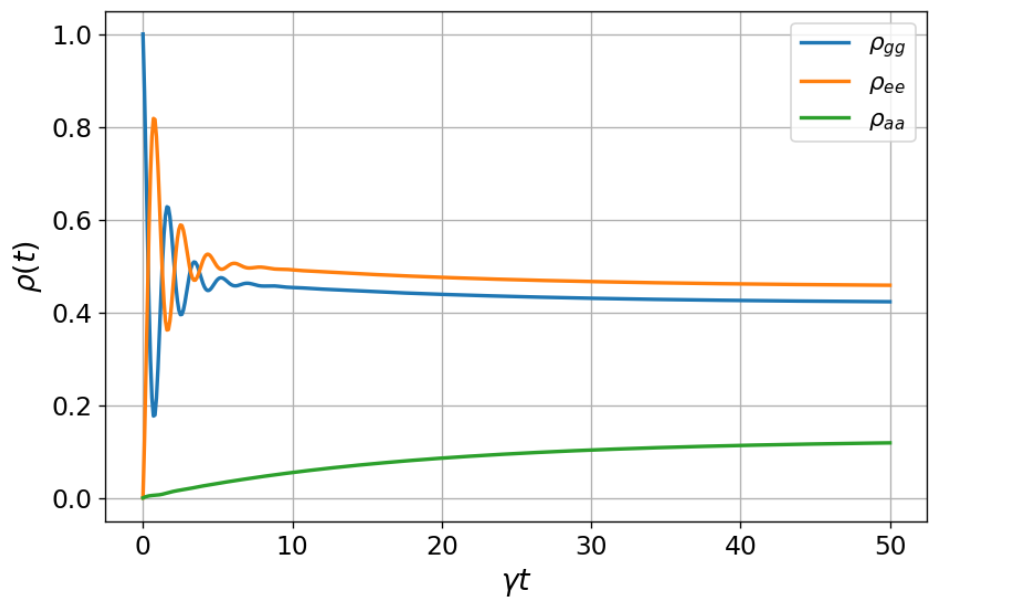
\includegraphics[width=0.8\textwidth]{imagenes/3lap(t).png}
    \caption{Evolución temporal de las poblaciones $p_{ee}(t)$, $p_{gg}(t)$ y $p_{aa}(t)$ con $\Omega = 3.5$, $\gamma = 1$, $\gamma_d = 0.05$ y $\gamma_a = 0.015$.}
    \label{fig:3la2omega}
\end{figure}

En primer lugar, se observa que la evolución de la población del estado excitado, $p_{ee}(t)$, contiene esencialmente toda la información relevante de la dinámica. Por esta razón, en las simulaciones posteriores nos centraremos principalmente en la evolución de esta población, o de manera equivalente, en la amplitud de probabilidad asociada al estado excitado.

Durante los tiempos cortos se aprecian oscilaciones de Rabi entre los estados $\ket{g}$ y $\ket{e}$, consecuencia de trabajar en el régimen $\Omega > \gamma$. Estas oscilaciones coherentes son las responsables de los picos laterales del triplete de Mollow observados en el espectro de fluorescencia. Sin embargo, debido a la disipación, dichas oscilaciones se amortiguan rápidamente y las poblaciones de los estados base y excitado comienzan a evolucionar de manera prácticamente paralela. Esta dinámica transitoria está asociada a la componente central inelástica del espectro de Mollow.

Finalmente, en escalas de tiempo más largas, el sistema exhibe una relajación lenta hacia un régimen cuasiestacionario determinado por la presencia del estado metaestable $\ket{a}$. Este proceso introduce una escala temporal mucho mayor que la asociada a las oscilaciones de Rabi y constituye una primera evidencia de la dinámica de *shelving*. Desde el punto de vista espectral, esta evolución lenta se manifiesta mediante la aparición de un pico central extremadamente angosto, característica distintiva de la fluorescencia resonante intermitente.

Aunque la ecuación maestra permite describir adecuadamente estas características promedio de la dinámica, no proporciona información directa sobre cómo se manifiestan en una realización individual del experimento. En particular, los períodos brillantes y oscuros asociados al fenómeno de \textit{shelving} surgen de manera natural al observar trayectorias individuales condicionadas por los resultados de medición del entorno. Esto motiva el empleo de ecuaciones de Schrödinger estocásticas y de la teoría de trayectorias cuánticas, las cuales constituyen una descripción complementaria a la ecuación maestra y permiten acceder a la dinámica microscópica subyacente a los promedios estadísticos.

Históricamente, las trayectorias estocásticas ofrecían una ventaja computacional clara frente a la integración de la ecuación maestra, debido a que la evolución de un estado puro de dimensión $d$ es mucho menos costosa que la evolución de un operador densidad de dimensión $d^2$.  
Aunque el aumento en la capacidad de cómputo moderna ha reducido esta diferencia para sistemas pequeños, existen actualmente numerosos casos donde las trayectorias siguen siendo superiores: sistemas de muchos cuerpos o de gran dimensión de Hilbert \cite{Daley2014,Lindner2022}, simulaciones paralelizables en GPU \cite{Li2022}, sistemas bosónicos o de circuit QED con grandes truncamientos \cite{Koch2019}, y dinámicas no-Markovianas donde la ecuación maestra resulta impracticable \cite{Suess2014,Ke2021}.

No obstante, para los propósitos del presente proyecto, la motivación principal para emplear trayectorias no es su posible eficiencia computacional, sino su \textbf{interpretación física como estados condicionados por resultados de medición}. Esta perspectiva proporciona una intuición directa sobre la relación entre la dinámica irreversible del sistema y los registros continuos o discretos del entorno, lo cual resulta central para el análisis conceptual desarrollado en este trabajo.







\section{Objetivos}
\textbf{Objetivo General:}

Simular sistemas cuánticos de dos y tres niveles mediante la Teoría de Trayectorias Cuánticas, en sus formulaciones de saltos cuánticos y trayectorias difusivas, con el propósito de estudiar el fenómeno de fluorescencia intermitente y extender el análisis al caso de bombeo incoherente. Como resultados principales se obtendrán la evolución de la función de onda, las poblaciones, la fotocorriente, la fotoestadística y los espectros de emisión.

\textbf{Objetivos Específicos:}

\begin{itemize}
    \item Simular un sistema de tres niveles con estructura de shelving bajo detección homodina, analizando cómo la dinámica estocástica se refleja en la fotocorriente y el espectro de fluorescencia en las cuadraturas $0$ y $\pi/2$, y demostrar que la suma de ambas cuadraturas reconstruye el espectro completo del triplete de Mollow.
    
    \item Desarrollar un análisis del fenómeno de fluorescencia intermitente con bombeo incoherente, mediante ecuación maestra y trayectorias de saltos cuánticos, comparando ambos enfoques y evaluando su consistencia.
    
    \item Obtener la evolución temporal de las poblaciones y compararlas con las soluciones de la ecuación maestra, utilizándolas como referencia para verificar la consistencia y precisión de las simulaciones estocásticas.
    
    \item Implementar simulaciones numéricas utilizando ecuaciones estocásticas diferenciales (SDEs) para trayectorias difusivas y algoritmos de saltos cuánticos para trayectorias discretas.

\end{itemize}

% Metodología
\section{Metodología}
\subsection{Trayectorias Cuánticas}
La intensidad, las correlaciones intensidad-intensidad, la distribución de tiempos de espera, la estadística de fotoelectrones y la estadística sub-Poissoniana se miden mediante conteo directo de fotones y se simulan mediante trayectorias discontinuas (saltos cuánticos). La detección homodina y heterodina, simuladas mediante trayectorias de difusión de estado cuántico, permiten mediciones de campo dependientes de la fase, como cuadratura única, compresión de ruido (squeezing) y espectros. La Detección Homodina Condicionada (CHD) combina saltos cuánticos y difusión cuántica para ofrecer una nueva perspectiva de las fluctuaciones cuánticas y resolver el squeezing de manera independiente de la eficiencia del detector. Los espectros pueden medirse mediante detección homodina, heterodina y mediciones filtradas \cite{TiCa92,Holland98}.

Las trayectorias cuánticas, tal como las formuló Carmichael, simulan la salida de un experimento, y un gran conjunto de trayectorias representa el resultado promedio de muchos experimentos.

\subsection{Detección Homodina Balanceada}

La detección homodina balanceada (DHB) es una técnica fundamental para la medición de ruido cuántico y, en particular, para la caracterización de \textit{estados comprimidos de la luz}. A diferencia de la detección heterodina, en este esquema el oscilador local (OL) tiene la misma frecuencia que el campo bajo estudio ($\omega_{\text{lo}} = \omega$). Ambos haces, el del emisor y el del OL, suelen provenir del mismo láser. La clave de este método reside en la capacidad de seleccionar la fase relativa $\phi$ del OL, lo que permite medir la varianza de una cuadratura específica del campo.

\subsubsection*{Principio de Operación}

El esquema de la DHB (ver Fig. \ref{fig:homodina_balanceada}) consiste en mezclar el modo del campo óptico de interés, $\hat{a}$, con el modo de un OL intenso y coherente, $\hat{b}$, en un divisor de haz (DH) balanceado ($R = T = 1/2$). Los modos de salida tras el divisor de haz están dados por:

\begin{eqnarray}
\hat{c} = \frac{1}{\sqrt{2}} (\hat{a} + i\hat{b}), \quad
\hat{d} = \frac{1}{\sqrt{2}} (i\hat{a} + \hat{b})
\end{eqnarray}

Las intensidades registradas en los fotodetectores D1 y D2 son proporcionales a $\hat{c}^\dagger \hat{c}$ y $\hat{d}^\dagger \hat{d}$, respectivamente. La esencia de la técnica ``balanceada'' es restar estas dos fotocorrientes para obtener la señal diferencia:

\begin{eqnarray}
\hat{n}_{cd} = \hat{c}^\dagger \hat{c} - \hat{d}^\dagger \hat{d} = -i(\hat{a}^\dagger \hat{b} - \hat{b}^\dagger \hat{a})
\label{eq:diferencia_corrientes}
\end{eqnarray}

Esta operación cancela el exceso de ruido clásico del OL, cuya intensidad es típicamente mucho mayor que la del emisor, permitiendo acceder a las fluctuaciones cuánticas del campo $\hat{a}$.

\subsubsection{Sensibilidad a las Cuadraturas}

Considerando que el OL se encuentra en un estado coherente de gran amplitud, $\hat{b} = \beta e^{i\phi}$, podemos aproximar $\hat{b}$ como un número complejo $\beta e^{i\phi}$. Sustituyendo en la Ecuación \ref{eq:diferencia_corrientes}, la señal medida se simplifica a:

\begin{eqnarray}
\hat{n}_{cd} = i\beta\left(\hat{a}^\dagger e^{i\phi} - \hat{a} e^{-i\phi}\right)
\end{eqnarray}

Manipulando algebraicamente esta expresión, se puede demostrar que es proporcional a un operador de cuadratura:

\begin{eqnarray}
\hat{n}_{cd} = 2\beta \hat{X}_{\phi + \pi/2} = 2\beta \hat{P}_{\phi}
\end{eqnarray}

donde $\hat{X}_{\theta} = \frac{1}{2}(\hat{a}^\dagger e^{i\theta} + \hat{a} e^{-i\theta})$ es el operador de cuadratura generalizado. Al normalizar por la amplitud del OL, la señal $\hat{n}_{cd}$ proporciona una medición directa de la cuadratura $\hat{P}_{\phi}$, que es la conjugada de $\hat{X}_{\phi}$. Variando la fase $\phi$ del OL, es posible medir cualquier cuadratura del campo, permitiendo así caracterizar completamente sus propiedades de ruido.

\subsubsection{Aplicaciones: Detección de Compresión}

La DHB es la técnica por excelencia para detectar estados comprimidos de la luz. Un estado está comprimido si la varianza de una de sus cuadraturas, $\Delta^2 \hat{X}_{\phi}$, es menor que el nivel de ruido del vacío (establecido como 1/4 en unidades adecuadas). Al medir el espectro de ruido de la fotocorriente diferencia $S(\omega, \phi)$, se puede obtener información sobre estas varianzas. Un valor de $S(\omega, \phi) < 1$ en una banda de frecuencias indica compresión, es decir, ruido cuántico por debajo del límite clásico.

\begin{figure}[h]
    \centering
    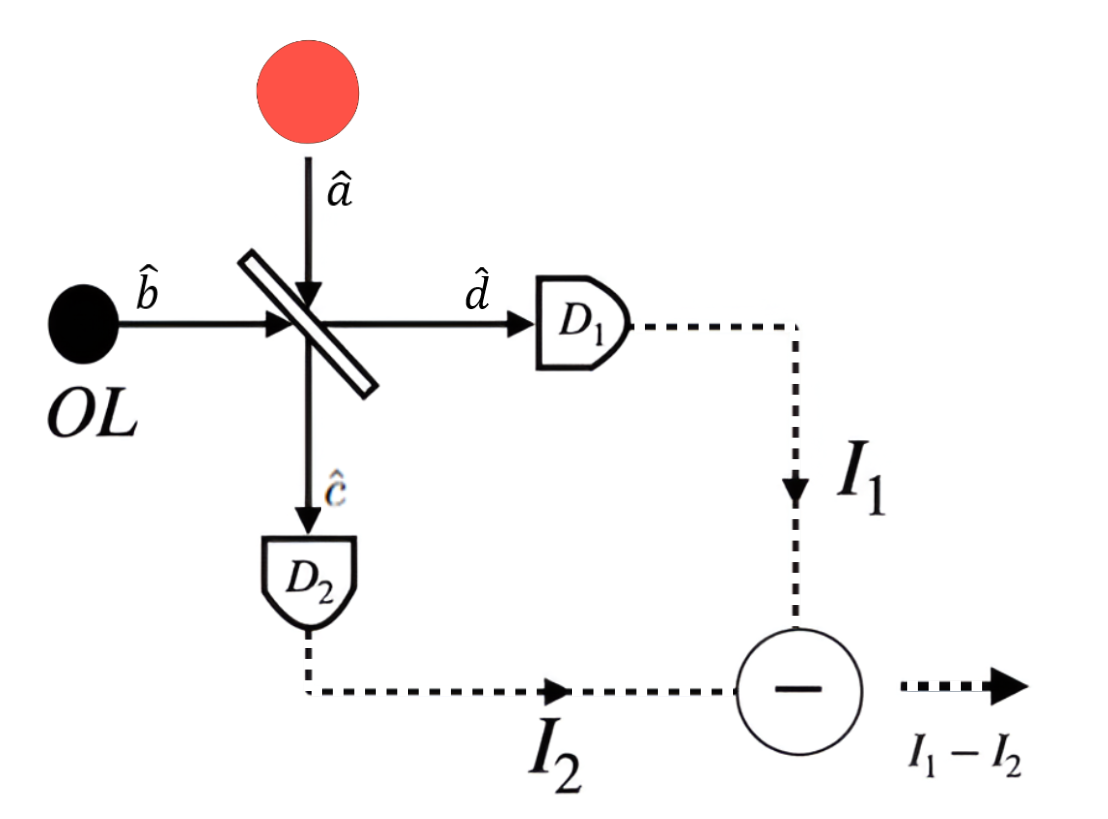
\includegraphics[width=0.7\linewidth]{imagenes/dhb.png}
    \caption{Esquema de detección homodina balanceada. Un mismo láser impulsa al emisor (círculo rojo) y al oscilador local (OL). Un elemento de fase (no mostrado) permite controlar la fase relativa $\phi$ para seleccionar la cuadratura a medir. La resta de las señales de los dos fotodetectores cancela el ruido clásico del OL.}
    \label{fig:homodina_balanceada}
\end{figure}

\subsubsection{EES para DHB en un átomo de tres niveles}

La EES que simula la detección homodina balanceada (DHB) para un átomo de tres niveles está dada por $i \hbar \ket{\dot{\bar{\Psi}}_c} = {\mcH}_W \ket{\bar{\Psi}_c}$ \cite{Carm93,WisemanMilburn2009}, donde

\begin{eqnarray} \label{eq:HamiltonianHDm_3L}
\mcH_W &=& \mcH + i \left(2 \gamma \langle \sigma_{\phi}^{eg} \rangle_c  
	+ \sqrt{\gamma} \,\eta_W(t) \right) e^{-i\phi}  \sigma_{eg} \,,
\end{eqnarray}

donde, para un átomo de tres niveles con estructura de shelving, el Hamiltoniano efectivo no Hermitiano y los operadores de salto se definen como

\begin{eqnarray}
\mcH &=& H_0 - i \frac{\gamma}{2} \sigma_{eg}\sigma_{ge}
      - i \frac{\gamma_d}{2} \sigma_{ae}\sigma_{ea}
      - i \frac{\gamma_a}{2} \sigma_{ga}\sigma_{ag} \,, \quad
\nonumber \\
H_0 &=& \hbar \Delta_g \sigma_{gg} + \hbar \Delta_a \sigma_{aa} + \hbar \Delta_e \sigma_{ee} 
      + \frac{\Omega}{2} (\sigma_{eg} + \sigma_{ge}) \,,
\nonumber \\ 
\sigma_{\phi}^{eg}  
&=& \frac{1}{2}(\bar{\sigma}_{ge} e^{i\phi} + \bar{\sigma}_{eg} e^{-i\phi} ) \,,
\end{eqnarray}

con los operadores definidos como

\begin{eqnarray}
\sigma_{eg} = \ket{e}\bra{g}, &\quad& \sigma_{ge} = \ket{g}\bra{e}, \nonumber \\
\sigma_{ae} = \ket{a}\bra{e}, &\quad& \sigma_{ea} = \ket{e}\bra{a}, \nonumber \\
\sigma_{ga} = \ket{g}\bra{a}, &\quad& \sigma_{ag} = \ket{a}\bra{g}, \nonumber \\
\sigma_{ee} = \ket{e}\bra{e}, &\quad& \sigma_{aa} = \ket{a}\bra{a}, \quad \sigma_{gg} = \ket{g}\bra{g}.
\end{eqnarray}

Aquí, $\gamma$ es la tasa de decaimiento $\ket{e} \to \ket{g}$, $\gamma_d$ es la tasa $\ket{e} \to \ket{a}$, y $\gamma_a$ es la tasa $\ket{a} \to \ket{g}$. El término $\eta_W = dW/dt$ es un ruido blanco Gaussiano y $dW$ es un incremento de Wiener real que satisface

\begin{equation} \label{eq:GaussianNoise_3L}
\overline{dW} = 0, \quad \overline{dW dW} = dt, \quad 
\overline{\eta_W(t) \eta_W(t')} = \delta(t-t').
\end{equation}

Podemos escribir la EES para DHB en un átomo de tres niveles como

\begin{subequations}
\begin{eqnarray}
\frac{d \ket{\bar{\Psi}_c}}{dt} 
	&=& \left\{ -i \mcH + I_c^W(t) \sigma_{eg} \right\} \ket{\bar{\Psi}_c}, \\
I_c^W(t) &=& \left(2 \gamma \langle \sigma_{\phi}^{eg} \rangle_c  
	+ \sqrt{\gamma} \,\eta_W(t) \right) e^{-i\phi} \\
&=& \gamma \left( \langle \bar{\sigma}_{ge} \rangle_c  
	+ e^{-2i\phi} \langle \bar{\sigma}_{eg} \rangle_c \right) 
	+ e^{-i\phi} \sqrt{\gamma} \, \eta_W(t), \nonumber 
\label{HomodyneSSE_3L}
\end{eqnarray}
\end{subequations}

donde $I_c^W$ es la fotocorriente medida en la detección homodina.

Vemos que la EES no es lineal debido a la presencia del valor esperado $\langle \sigma_{\phi}^{eg} \rangle$ y que no contiene directamente información de la intensidad y frecuencia del láser. Aparte de la fase $\phi$, el láser se presenta en la forma en que la estocasticidad entra: en lugar de evaluar si se registró un fotoelectrón o no cada $dt$, ahora hay muchos fotoelectrones en dicho intervalo, produciendo un cambio continuo e infinitesimal en la función de onda. No sería práctico hacer $dt$ demasiado pequeño comparado con el inverso de la razón de fotoconteo. Entonces, más que fotoelectrones aislados, se tiene una fotocorriente cuyas fluctuaciones tienen un carácter diferente al de fotoconteo: pasamos de ruido Poissoniano o sub-Poissoniano a ruido Gaussiano. 

Una vez obtenida la fotocorriente $I_c^W(t)$ a partir de la simulación de la EES, el siguiente paso natural es caracterizar sus propiedades estadísticas. La función de autocorrelación de la fotocorriente, definida como $\overline{I_c(t+\tau) I_c(t)}$, proporciona información fundamental sobre las fluctuaciones de la señal detectada y su relación con la dinámica atómica subyacente. Utilizando el teorema de regresión cuántica de Onsager-Lax, junto con las propiedades del ruido Gaussiano dadas en la Ec.~\eqref{eq:GaussianNoise_3L}, se obtiene la siguiente expresión para la autocorrelación \cite{WisemanMilburn2009}:

\begin{eqnarray} \label{HomodyneAutoCorr_3L}
\overline{ I_c(t+\tau) I_c(t) } &=& \gamma^2 
	\langle : \sigma_{\phi}^{eg} (t+\tau) \sigma_{\phi}^{eg} (t) : \rangle 
	+\gamma \delta (\tau), \qquad
\end{eqnarray}

donde los dos puntos indican ordenamiento normal y $\langle \cdots \rangle$ denota el promedio en el estado estacionario. El primer término contiene las correlaciones atómicas, mientras que el segundo, proporcional a $\gamma \delta(\tau)$, corresponde al ruido shot noise característico de la detección homodina. El espectro de fluorescencia se obtiene calculando la transformada de Fourier de esta correlación,

\begin{eqnarray} \label{SpectrumHom_3L}
S(\omega,\phi)-1 \propto \gamma \int_0^{\infty} d\tau\, \cos(\omega \tau) 
	\langle : \sigma_{\phi}^{eg} (t+\tau) \sigma_{\phi}^{eg} (t) : \rangle.
\end{eqnarray}.


\subsection{Reemplazando el Láser por un Campo Incoherente}

La observación de la intermitencia no requiere estrictamente una excitación atómica coherente. La excitación incoherente, como la de un láser operando por debajo del umbral, también puede inducir fluorescencia intermitente. Aquí, retomamos el modelo estudiado en la Introducción de semestres anteriores y reemplazamos el láser que excita la transición $|g\rangle - |e\rangle$ por un campo incoherente de banda ancha \ref{fig:3nivelesinc}. En lugar del Hamiltoniano átomo-láser, tenemos ahora un nuevo término en el Liouvillian que describe este tipo de excitación, que puede interpretarse en cierta medida como radiación de cuerpo negro con número promedio de fotones $\bar{n} = [e^{\hbar \omega/k_BT} -1]^{-1}$. El esquema de emisión espontánea es el mismo que en el problema con láser. Además, debido al ancho de banda, no hay desintonía.

\begin{figure}[H]
    \centering
    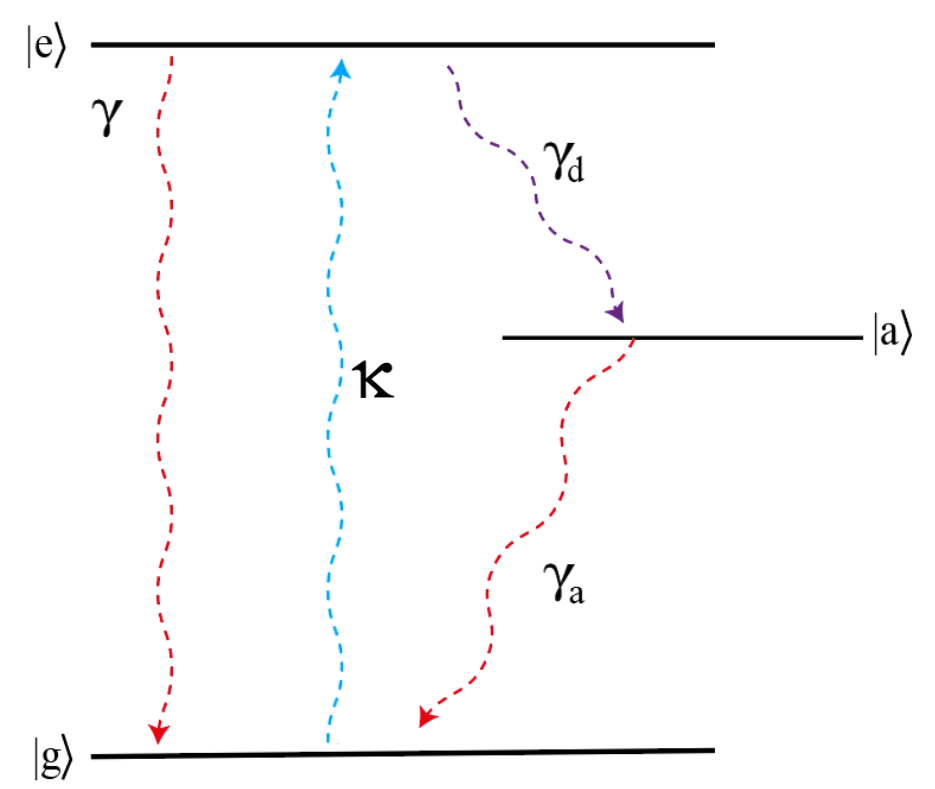
\includegraphics[width=0.5\textwidth]{imagenes/3LAinch.png}
    \caption{Esquema de niveles atómicos con bombeo incoherente representado con la letra $\kappa$ y decaimiento radiativo.}
    \label{fig:3nivelesinc}
\end{figure}

En nuestro modelo, en lugar de asumir un campo con temperatura $T \neq 0$, introducimos una tasa de excitación incoherente $\kappa = \gamma \bar{n}/2$ y hacemos la sustitución $\gamma (\bar{n}+1)/2 \to \gamma/2$. El efecto neto es reemplazar el término $-(i/\hbar) [H,\rho]$ por

\begin{eqnarray}
\mathcal{L}_B \rho &=& \kappa [ 2\sigma_{eg} \rho \sigma_{ge} 
	-\sigma_{ge} \sigma_{eg} \rho -\rho \sigma_{ge} \sigma_{eg} ] 	
	\qquad
\end{eqnarray}

%%%%%%%%%%%%%%%%%%%%%%%
\subsubsection{Átomo de Dos Niveles con Bombeo Incoherente}

La ecuación maestra para un átomo de dos niveles bajo excitación incoherente está dada por

\begin{eqnarray}
\dot{\rho}(t) &=&  \kappa (2\sigma_{eg} \rho \sigma_{ge} 
  	-\sigma_{ge} \sigma_{eg} \rho  -\rho \sigma_{ge} \sigma_{eg})     
  	\nonumber \\
&&+\frac{\gamma}{2} (2\sigma_{ge} \rho \sigma_{eg} 
  	-\sigma_{eg} \sigma_{ge} \rho  -\rho \sigma_{eg} \sigma_{ge})     
\end{eqnarray}

De aquí obtenemos las ecuaciones de evolución para las poblaciones:

\begin{subequations}
\begin{eqnarray}
\dot{\rho}_{ee} &=& 2\kappa \rho_{gg} -\gamma \rho_{ee} \,, \\ 
\dot{\rho}_{gg} &=& -2\kappa \rho_{gg} +\gamma \rho_{ee} \,, 
\end{eqnarray}
\end{subequations}

con $\rho_{ee} + \rho_{gg} = 1$. Imponiendo la condición de estado estacionario ($\dot{\rho}_{ee} = \dot{\rho}_{gg} = 0$), obtenemos

\begin{subequations}
\begin{eqnarray}
\rho_{ee}^{st} &=& \frac{2\kappa}{2\kappa + \gamma} \,, \\
\rho_{gg}^{st} &=& \frac{\gamma}{2\kappa + \gamma} \,. 
\end{eqnarray}
\end{subequations}

Estas soluciones muestran que la población excitada aumenta con la tasa de bombeo $\kappa$ y disminuye con la tasa de decaimiento $\gamma$, como era de esperarse.
%%%%%%%%%%%%%%%%%%%%%%%
\subsubsection{Átomo de Tres Niveles con Bombeo Incoherente}

la ecuación maestra para el átomo de tres niveles está dada por

\begin{eqnarray}
\dot{\rho}(t) &=&  \kappa (2\sigma_{eg} \rho \sigma_{ge} 
  	-\sigma_{ge} \sigma_{eg} \rho  -\rho \sigma_{ge} \sigma_{eg})     
  	\nonumber \\
&&+\frac{\gamma}{2} (2\sigma_{ge} \rho \sigma_{eg} 
  	-\sigma_{eg} \sigma_{ge} \rho  -\rho \sigma_{eg} \sigma_{ge})     
  	\nonumber \\
&& + \frac{\gamma_d}{2} (2\sigma_{ae} \rho \sigma_{ea} 
  	-\sigma_{ea} \sigma_{ae} \rho -\rho \sigma_{ea} \sigma_{ae}) 	
	\nonumber \\ 
&& +\frac{\gamma_a}{2} (2\sigma_{ga} \rho \sigma_{ag} 
  	-\sigma_{ag} \sigma_{ga} \rho  -\rho \sigma_{ag} \sigma_{ga}) \,, 
	\qquad
\end{eqnarray}

que puede simplificarse como

\begin{eqnarray}
\dot{\rho}(t) &=& \kappa ( 2 \rho_{gg} \sigma_{ee} -\sigma_{gg} \rho 
	-\rho \sigma_{gg} ) 	\nonumber \\
&& -\frac{\gamma_+}{2} (\sigma_{ee} \rho +\rho \sigma_{ee}) 
    -\frac{\gamma_a}{2} (\sigma_{aa} \rho +\rho \sigma_{aa}) 
        \nonumber \\
&& +\gamma \rho_{ee} \sigma_{gg}  +\gamma_d \rho_{ee} \sigma_{aa}    
    +\gamma_a \rho_{aa} \sigma_{gg}  \,.  \qquad \qquad  
    \label{masterEqInc}
\end{eqnarray}

Nos quedamos con ecuaciones para las poblaciones únicamente, ya que las coherencias se anulan. Además, estas últimas son cero en todo momento,

\begin{subequations}
\begin{eqnarray}
\dot{\rho}_{ee} &=& 2\kappa \rho_{gg} -\gamma_+ \rho_{ee} 	\,, \\ 
\dot{\rho}_{gg} &=& -2\kappa \rho_{gg} +\gamma \rho_{ee} 
	+\gamma_a \rho_{aa} 	\,, \\  
\dot{\rho}_{aa} &=& \gamma_d \rho_{ee} -\gamma_a \rho_{aa} 	\,.
\end{eqnarray}
\end{subequations}

Estas son \textit{ecuaciones de tasas}, que describen el flujo de poblaciones entre los niveles. De hecho, el primer estudio teórico de la fluorescencia resonante intermitente (para un átomo de tres niveles en configuración V) utilizó ecuaciones de tasas en lugar de ecuaciones de Bloch \cite{CoKi86}.

Las soluciones en estado estacionario (donde $\dot{\rho}_{jj} = 0$) son:

\begin{subequations}
\begin{eqnarray}
\rho_{ee}^{st} &=& \frac{ 2\kappa \gamma_a }
		{ \gamma_+ \gamma_a +2\kappa (\gamma_d +\gamma_a) } \,, \\
\rho_{gg}^{st} &=& \frac{ \gamma_+ \gamma_a }
		{ \gamma_+ \gamma_a +2\kappa (\gamma_d +\gamma_a) } \,, \\ 
\rho_{aa}^{st} &=& \frac{ 2\kappa \gamma_d }
		{ \gamma_+ \gamma_a +2\kappa (\gamma_d +\gamma_a) } \,. 
		\qquad
\end{eqnarray}
\end{subequations}

La matriz para este sistema es

\begin{eqnarray}
\mathbf{M}_{B} = \left( \begin{array}{ccc} 
	-\gamma_+ & 2\kappa & 0 \\ 
	\gamma & -2\kappa &\gamma_a \\
	\gamma_d & 0 & \gamma_a  \end{array}  \right) \,.  \qquad 
\end{eqnarray}

y el vector es $\mathbf{r}_{B} = \left( \rho_{ee}, \rho_{gg}, \rho_{aa} \right)^T$. Nótese que el sistema de ecuaciones es homogéneo.

%%%%%%%%%%%%%%%%%%%%%%%%%%%%%%%%
\subsubsection{Reducción Adicional del Sistema de Ecuaciones}

Usando la conservación de la población, $\rho_{aa} = 1 - \rho_{ee} - \rho_{gg}$, el sistema de ecuaciones se reduce a

\begin{subequations}
\begin{eqnarray}
\dot{\rho}_{ee} &=& 2\kappa \rho_{gg} -\gamma_+ \rho_{ee} 	\,, \\ 
\dot{\rho}_{gg} &=& -(2\kappa +\gamma_a) \rho_{gg} 
	+\gamma_- \rho_{ee} +\gamma_a  	 	\, \qquad
\end{eqnarray}
\end{subequations}

donde $\gamma_- = \gamma - \gamma_a$.

Estas ecuaciones pueden escribirse en forma matricial:

\begin{eqnarray}
\dot{\mathbf{q}}(t) = \mathbf{M}_C \mathbf{q}(0) +\mathbf{g} 	\,,
\end{eqnarray}

donde

\begin{eqnarray}
\mathbf{q} = \left( \begin{array}{c} \rho_{ee} \\ \rho_{gg} \end{array}  \right) \,, 
	\qquad \qquad
\mathbf{g} = \left( \begin{array}{c} 0 \\ \gamma_a \end{array}  \right) \,, \\
\mathbf{M}_C = \left( \begin{array}{cc} -\gamma_+ & 2\kappa \\ 
	\gamma_- & -(2\kappa +\gamma_a)  \end{array}  \right) \,.  
\end{eqnarray}

Usando Mathematica, con la opción FullSimplify, los valores propios de $\mathbf{M}_C$ resultan ser

\begin{subequations}
\begin{eqnarray}
\lambda_{\pm} &=& - \frac{2\kappa +\gamma_+ +\gamma_a}{2} \nonumber \\
	&&\pm \frac{1}{2} 
	\sqrt{ 8\kappa \gamma_- +(2\kappa -\gamma_+ +\gamma_a)^2  } \,, 
	\qquad \\
\lambda_+ &\gg& \lambda_- \,.  
\end{eqnarray}
\end{subequations}

$\lambda_+$ representa el decaimiento rápido y $\lambda_-$ el decaimiento lento causante de la intermitencia de la fluorescencia.

$$ f(t) = A e^{\lambda_+ t} + B e^{\lambda_- t} .$$


%%%%%%%%%%%%%%%%%%%%%%%%%%
\subsubsection{Modelo Estocástico para Fluorescencia Intermitente}

Para describir estadísticamente la alternancia entre periodos brillantes y oscuros, recurrimos al formalismo de trayectorias de saltos cuánticos, siguiendo el enfoque de Carmichael. Este modelo permite obtener las distribuciones de tiempos de los periodos brillantes y oscuros, así como las probabilidades asociadas a cada régimen.

En primer lugar, consideramos la dinámica del estado metaestable $\ket{a}$, cuya evolución está gobernada por la ecuación de tasas

\begin{equation}
\dot{\rho}_{aa} = \gamma_d \rho_{ee} - \gamma_a \rho_{aa}.
\end{equation}

Durante un periodo oscuro, el átomo se encuentra atrapado en el estado $\ket{a}$, de modo que $\rho_{aa}(0) \approx 1$ y $\rho_{ee}(0) \approx 0$. El tiempo promedio de duración del periodo oscuro está determinado por la derivada inicial de $\rho_{aa}$,

\begin{equation}
T_D^{-1} = -(\dot{\rho}_{aa})_{t=0} = \gamma_a,
\end{equation}

lo que conduce a un tiempo promedio de duración del periodo oscuro dado por

\begin{equation}
T_D = \gamma_a^{-1}.
\end{equation}

Este resultado es intuitivo: mientras más grande sea la tasa de decaimiento $\gamma_a$ del estado metaestable al fundamental, más cortos serán los periodos oscuros.

Por otro lado, durante un periodo brillante, el átomo se encuentra fuera del estado metaestable, por lo que $\rho_{aa}(0) = 0$ y $\rho_{ee}(0)$ toma el valor estacionario correspondiente al subsistema de dos niveles $\ket{g} - \ket{e}$. Para el caso de excitación incoherente, este valor está dado por

\begin{equation}
\rho_{ee}^{st,(2LA)} = \frac{2\kappa}{2\kappa + \gamma},
\end{equation}

que representa la población excitada en el régimen brillante antes de que ocurra una transición al estado metaestable. El tiempo promedio de duración del periodo brillante se obtiene entonces como

\begin{equation}
T_B^{-1} = (\dot{\rho}_{aa})_{t=0} = \gamma_d \rho_{ee}^{st,(2LA)} = \gamma_d \frac{2\kappa}{2\kappa + \gamma}.
\end{equation}

Por lo tanto, el tiempo promedio de duración de un periodo brillante es

\begin{equation}
T_B = \frac{2\kappa + \gamma}{2\kappa \gamma_d}.
\end{equation}

Este resultado muestra que $T_B$ depende tanto de la tasa de bombeo incoherente $\kappa$ como de la tasa de decaimiento $\gamma_d$ hacia el estado metaestable.

Finalmente, las distribuciones de tiempos $P_B$ y $P_D$ pueden obtenerse a partir de los tiempos promedio calculados. En el caso más simple, estas distribuciones son exponenciales,

\begin{equation}
P_B(t) = T_B^{-1} e^{-t/T_B}, \qquad P_D(t) = T_D^{-1} e^{-t/T_D},
\end{equation}

lo que permite comparar directamente las predicciones teóricas con los histogramas obtenidos de las simulaciones numéricas mediante trayectorias de saltos cuánticos.
\section{Resultados:Detección Homodina Balanceada }

\subsection{Trayectorias Individuales y Fotocorriente}

En la Figura~\ref{fig:trayectorias_cuadraturas} se muestra la evolución temporal de la amplitud de probabilidad del estado excitado y la fotocorriente $I_c(t)$ para una trayectoria cuántica individual bajo detección homodina balanceada, en las cuadraturas $\theta = 0$ y $\theta = \pi/2$. 

La amplitud de probabilidad del estado excitado presenta fluctuaciones características de la dinámica estocástica del sistema. En la cuadratura $\theta = \pi/2$, se observa un cambio abrupto en la amplitud, el cual indica una transición hacia el estado metaestable $\ket{a}$, dando inicio a un periodo oscuro. Durante este intervalo, la emisión de fluorescencia cesa y el átomo permanece atrapado en dicho estado hasta que decae espontáneamente al estado fundamental.

Por su parte, la fotocorriente $I_c(t)$ registrada en ambas cuadraturas muestra fluctuaciones continuas alrededor de un valor medio. En particular, en la cuadratura $\theta = \pi/2$ se aprecia que, si bien la señal presenta ruido, su promedio temporal tiende a cero, lo cual es consistente con la ausencia de emisión coherente durante los periodos oscuros. Este comportamiento refleja la naturaleza estocástica del proceso de detección y la pérdida de coherencia asociada al atrapamiento en el estado metaestable.

\begin{figure}[H]
    \centering
    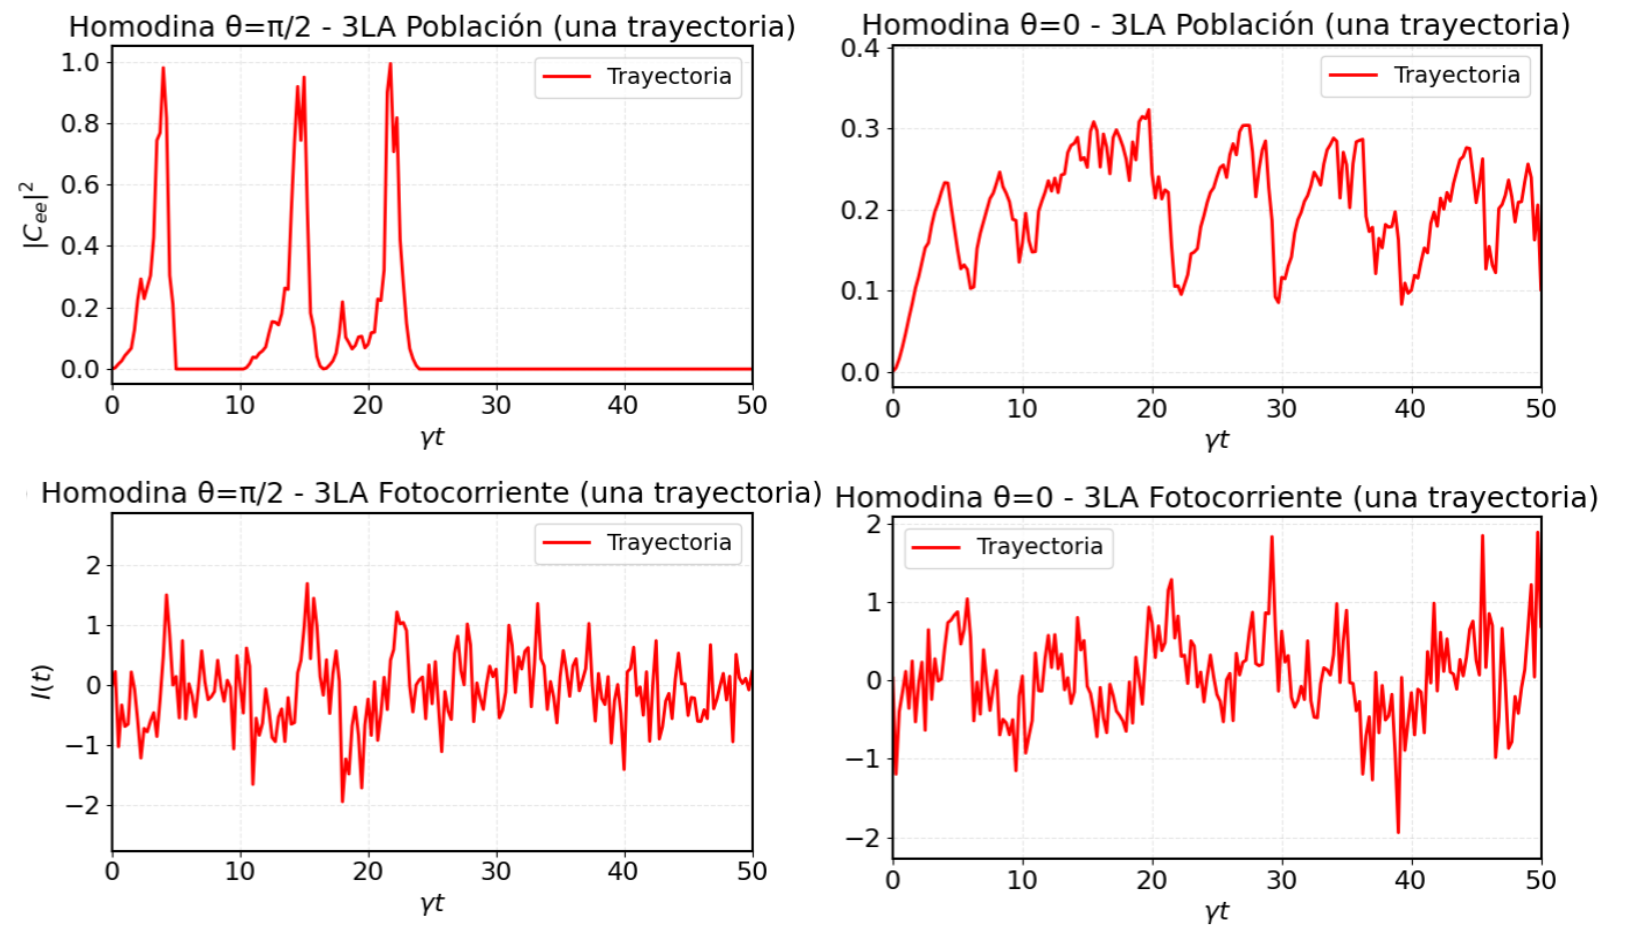
\includegraphics[width=0.9\textwidth]{imagenes/tr1homodina.png}
    \caption{Evolución temporal de la amplitud de probabilidad del estado excitado y la fotocorriente $I_c(t)$ para una trayectoria cuántica individual bajo detección homodina balanceada en las cuadraturas $\theta = 0$ y $\theta = \pi/2$.}
    \label{fig:trayectorias_cuadraturas}
\end{figure}


\subsection{Promedio sobre 500 Trayectorias}

En la Figura~\ref{fig:promedio_500_trayectorias} se presenta el promedio de 500 trayectorias cuánticas para la fotocorriente $I_c(t)$ y la amplitud de probabilidad del estado excitado, en las cuadraturas $\theta = 0$ y $\theta = \pi/2$.

Al promediar sobre un conjunto de 500 trayectorias, el ruido estadístico característico de las realizaciones individuales se reduce considerablemente, dando lugar a señales más suaves y representativas del comportamiento promedio del sistema. En el caso de la fotocorriente, el promedio en ambas cuadraturas revela una estructura que refleja diferentes componentes del espectro de fluorescencia. La cuadratura $\theta = 0$ está asociada al pico central coherente, mientras que la cuadratura $\theta = \pi/2$ corresponde a los picos laterales del triplete de Mollow. De manera análoga, el promedio de la amplitud de probabilidad del estado excitado presenta formas distintas en cada cuadratura, pero ambas contribuyen a reconstruir la evolución temporal obtenida a partir de la ecuación maestra. Esta correspondencia confirma que el promedio sobre un número suficiente de trayectorias reproduce la dinámica determinista del sistema, validando así la consistencia del enfoque estocástico.

\begin{figure}[H]
    \centering
    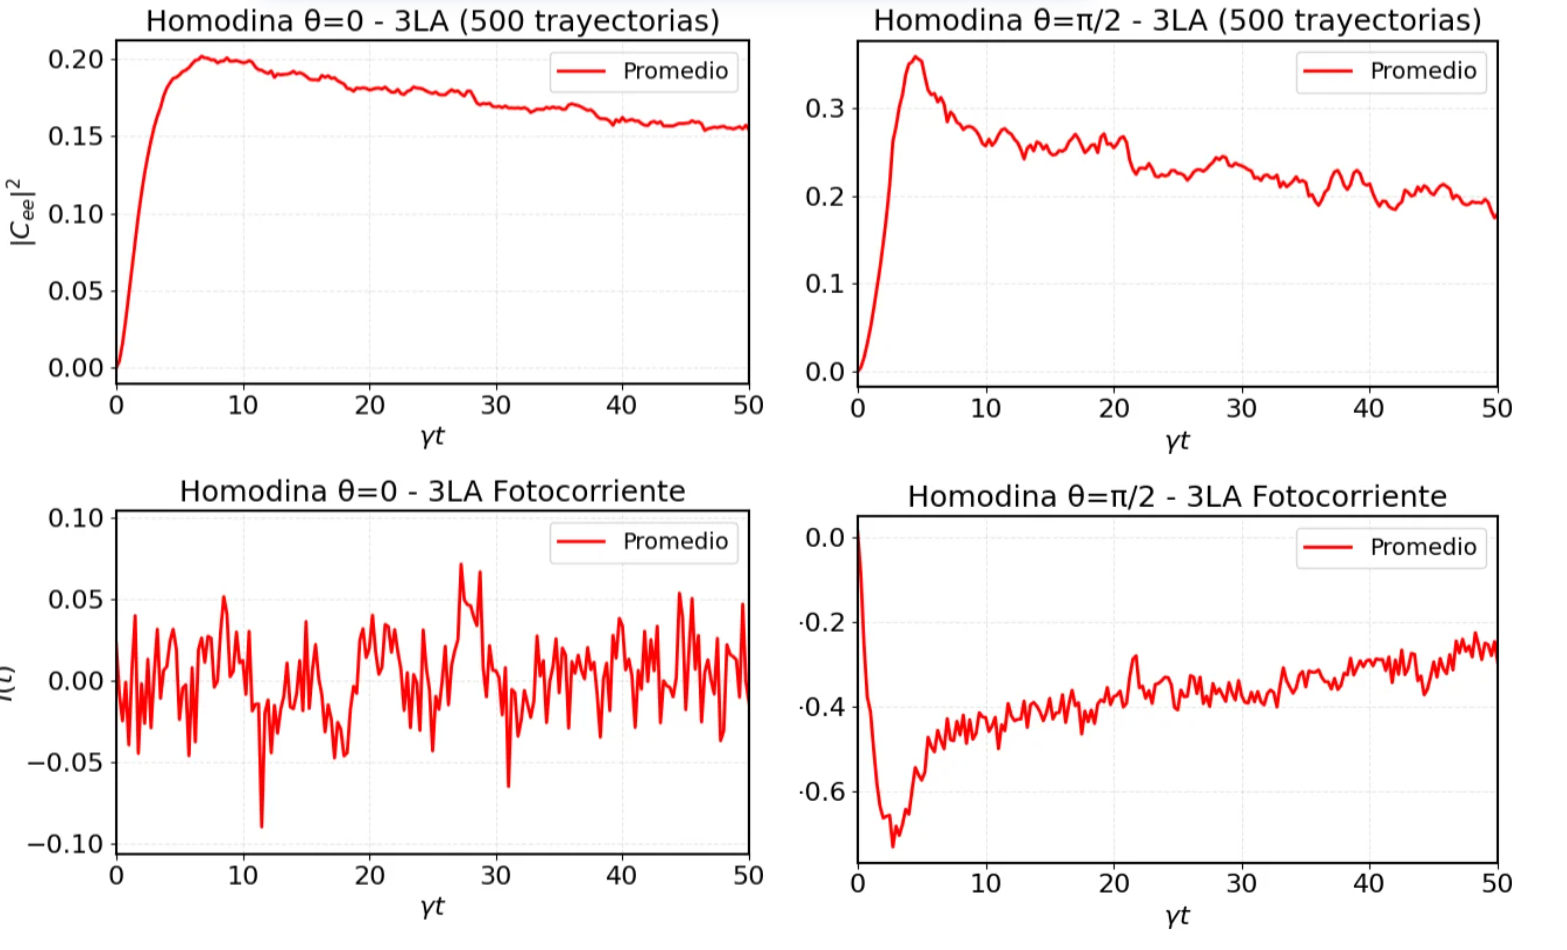
\includegraphics[width=0.9\textwidth]{imagenes/tr500.png}
    \caption{Promedio de 500 trayectorias cuánticas para la fotocorriente $I_c(t)$ y la amplitud de probabilidad del estado excitado en las cuadraturas $\theta = 0$ y $\theta = \pi/2$.}
    \label{fig:promedio_500_trayectorias}
\end{figure}

\subsection{Espectros de Fluorescencia a partir de la Autocorrelación}

Finalmente, en la Figura~\ref{fig:espectros_autocorrelacion} se presentan las funciones de autocorrelación de las fotocorrientes promedio y sus correspondientes espectros de fluorescencia para las cuadraturas $\theta = 0$ y $\theta = \pi/2$. Los espectros se obtienen calculando la transformada de Fourier de la función de autocorrelación de la fotocorriente, de acuerdo con la relación

\begin{equation}
S(\omega, \theta) \propto \int_{-\infty}^{\infty} d\tau \, e^{-i\omega \tau} \overline{I_c(t+\tau) I_c(t)}.
\end{equation}

En la cuadratura $\theta = 0$, el espectro presenta el pico central coherente característico del triplete de Mollow, asociado a la emisión elástica del campo láser. Por otro lado, en la cuadratura $\theta = \pi/2$, el espectro revela los picos laterales inelásticos del triplete, así como el pico angosto correspondiente al efecto de shelving, el cual surge de la dinámica lenta asociada al estado metaestable. Ambas cuadraturas proporcionan información complementaria: mientras que una captura la componente coherente de la emisión, la otra revela las contribuciones incoherentes y la estructura fina del espectro.

\begin{figure}[H]
    \centering
    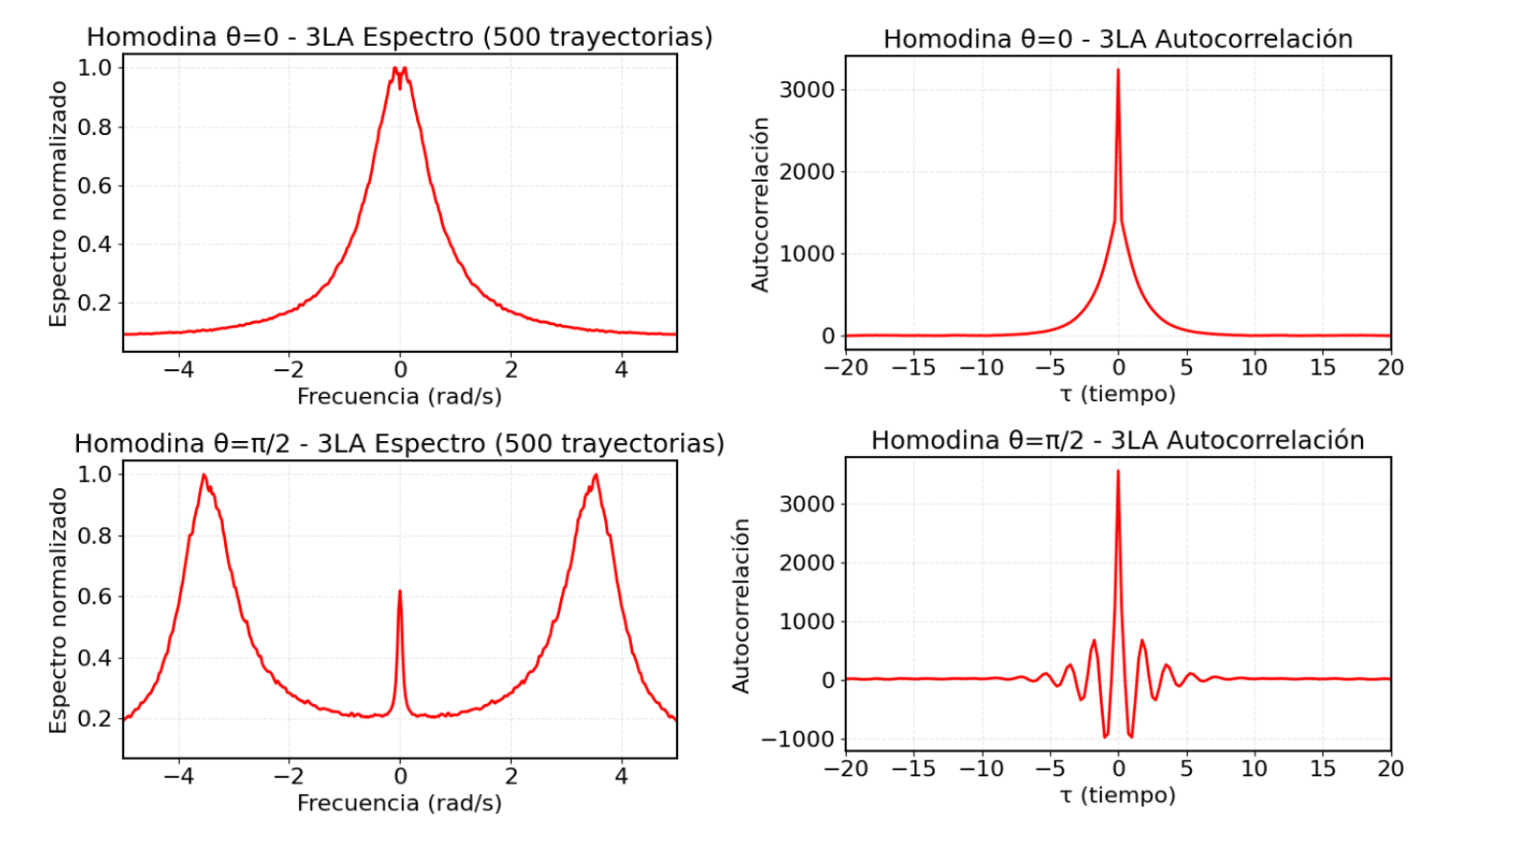
\includegraphics[width=0.9\textwidth]{imagenes/espectro autocorr.png}
    \caption{Funciones de autocorrelación de las fotocorrientes promedio y espectros de fluorescencia correspondientes para las cuadraturas $\theta = 0$ y $\theta = \pi/2$. Los espectros se obtienen mediante la transformada de Fourier de la autocorrelación.}
    \label{fig:espectros_autocorrelacion}
\end{figure}

La combinación de ambas cuadraturas permite reconstruir el espectro completo de fluorescencia, donde el pico central coherente y los picos laterales inelásticos, junto con el pico angosto del shelving, conforman la estructura total del triplete de Mollow modificado por la presencia del estado metaestable. Este resultado demuestra que la detección homodina balanceada, junto con el análisis de autocorrelación, constituye una herramienta poderosa para descomponer y estudiar las diferentes contribuciones espectrales en sistemas de tres niveles con fluorescencia intermitente.




\section{Resultados: Bombeo Incoherente}


\subsection{Estado Estacionario en Función de $\kappa/\gamma$}

En la Figura~\ref{fig:estado_estacionario_kappa} se muestra la solución del operador densidad en estado estacionario para el átomo de tres niveles bajo excitación incoherente, en función de la tasa de bombeo $\kappa$ normalizada por la tasa de decaimiento $\gamma$. Las poblaciones estacionarias $\rho_{ee}^{st}$, $\rho_{gg}^{st}$ y $\rho_{aa}^{st}$ están dadas por las ecuaciones

\begin{subequations}
\begin{eqnarray}
\rho_{ee}^{st} &=& \frac{2\kappa \gamma_a}{\gamma_+ \gamma_a + 2\kappa(\gamma_d + \gamma_a)}, \\
\rho_{gg}^{st} &=& \frac{\gamma_+ \gamma_a}{\gamma_+ \gamma_a + 2\kappa(\gamma_d + \gamma_a)}, \\
\rho_{aa}^{st} &=& \frac{2\kappa \gamma_d}{\gamma_+ \gamma_a + 2\kappa(\gamma_d + \gamma_a)}.
\end{eqnarray}
\end{subequations}

En el límite de bombeo débil ($\kappa \ll \gamma$), la población del estado fundamental $\rho_{gg}^{st}$ domina, mientras que las poblaciones de los estados excitado $\rho_{ee}^{st}$ y metaestable $\rho_{aa}^{st}$ son prácticamente nulas. A medida que $\kappa$ aumenta, $\rho_{ee}^{st}$ y $\rho_{aa}^{st}$ crecen, alcanzando valores de saturación determinados por las tasas de decaimiento $\gamma_d$ y $\gamma_a$. En particular, $\rho_{aa}^{st}$ tiende a un valor constante cuando el bombeo incoherente es suficientemente intenso, reflejando el balance entre la excitación hacia el estado metaestable y su decaimiento al estado fundamental.

\begin{figure}[H]
    \centering
    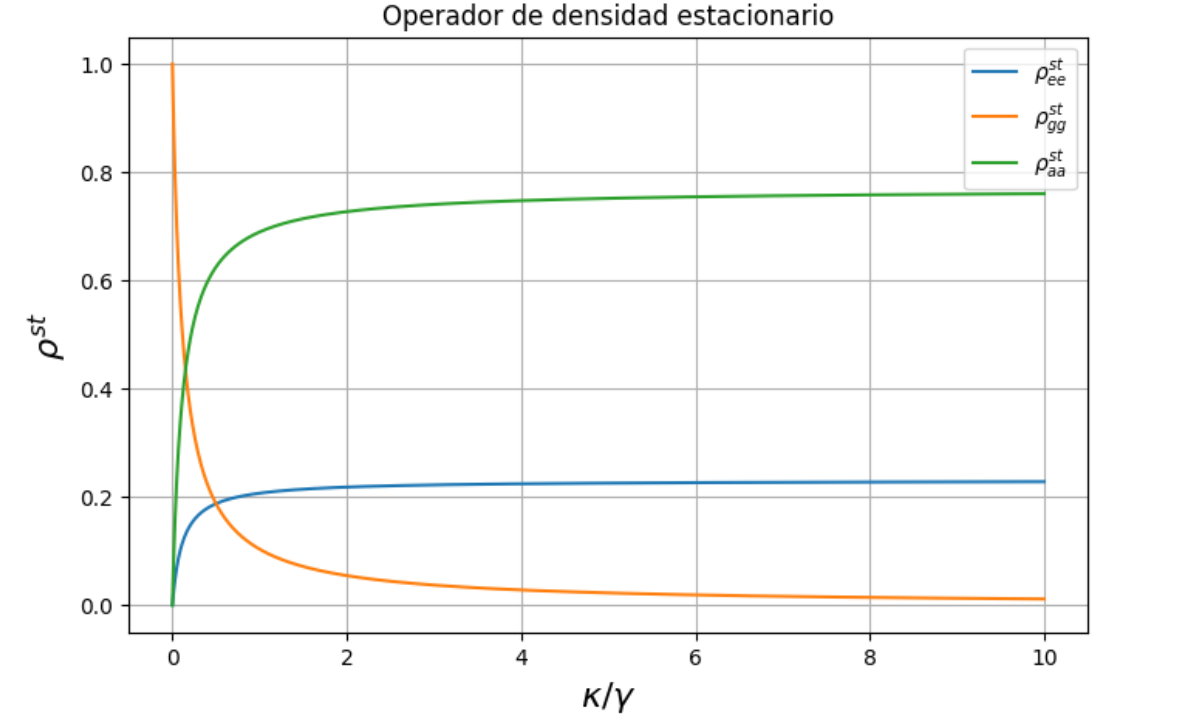
\includegraphics[width=0.8\textwidth]{imagenes/pst3lainch.png}
    \caption{Poblaciones estacionarias $\rho_{ee}^{st}$, $\rho_{gg}^{st}$ y $\rho_{aa}^{st}$ en función de $\kappa/\gamma$ para el átomo de tres niveles con bombeo incoherente.}
    \label{fig:estado_estacionario_kappa}
\end{figure}
\subsubsection{Comparación con Excitación Coherente}

En la Figura~\ref{fig:comparacion_coh_incoh} se comparan las evoluciones temporales de las poblaciones del estado excitado $\rho_{ee}(t)$ y del estado metaestable $\rho_{aa}(t)$ para los casos de excitación coherente (láser) e incoherente (bombeo). Ambas simulaciones se realizaron resolviendo numéricamente la ecuación maestra con QuTiP para el átomo de tres niveles.

En el caso de excitación coherente, la población $\rho_{ee}(t)$ presenta oscilaciones de Rabi características, que reflejan la coherencia inducida por el campo láser. Estas oscilaciones se amortiguan gradualmente debido a los decaimientos espontáneos y al acoplamiento con el estado metaestable, hasta alcanzar el estado estacionario. Por otro lado, en el caso de excitación incoherente, la dinámica es puramente disipativa y monótona: $\rho_{ee}(t)$ crece desde cero y se satura sin oscilar, ya que el bombeo incoherente no introduce coherencias en el sistema.

\begin{figure}[H]
    \centering
    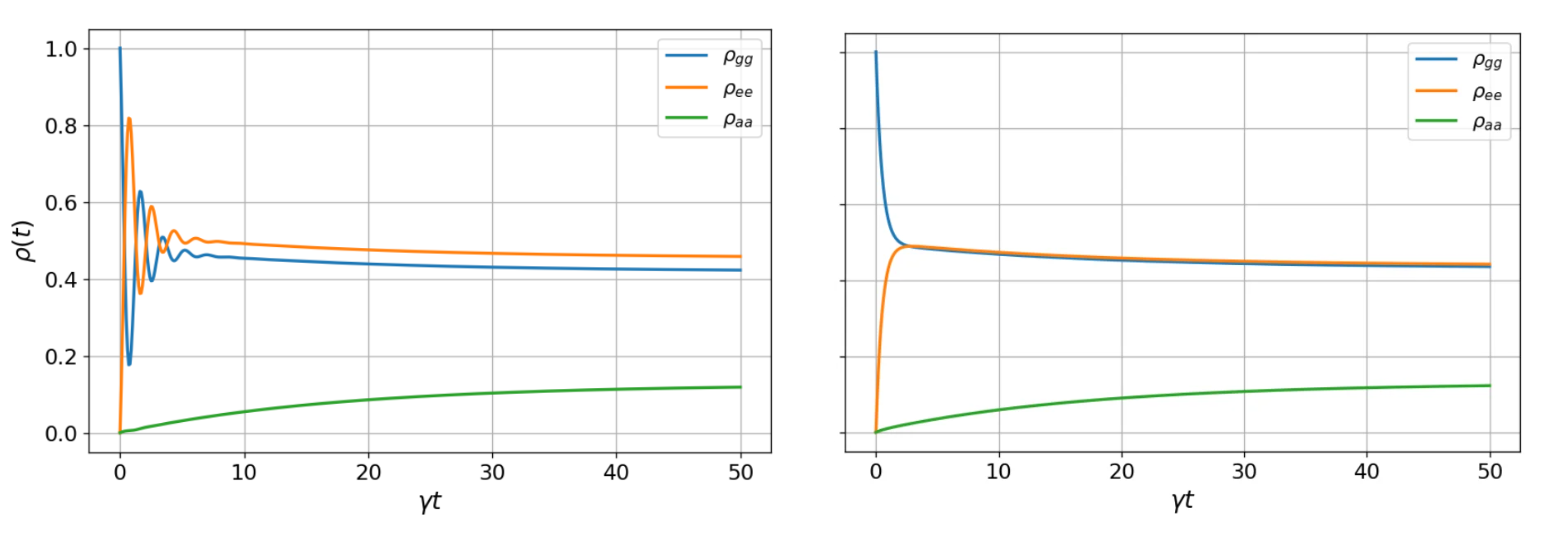
\includegraphics[width=1\textwidth]{imagenes/cohinc.png}
    \caption{Comparación de la evolución temporal de las poblaciones $\rho_{ee}(t)$ y $\rho_{aa}(t)$ para excitación coherente (láser) e incoherente (bombeo). La excitación coherente presenta oscilaciones de Rabi, mientras que la excitación incoherente exhibe una dinámica monótona.}
    \label{fig:comparacion_coh_incoh}
\end{figure}

En cuanto al estado metaestable $\rho_{aa}(t)$, en ambos casos se observa un crecimiento progresivo hacia el valor estacionario. Sin embargo, en la excitación coherente, $\rho_{aa}(t)$ también presenta pequeñas oscilaciones amortiguadas acopladas a la dinámica de $\rho_{ee}(t)$, mientras que en el caso incoherente el crecimiento es suave y monótono. Esta diferencia refleja el papel de las coherencias en el sistema: la excitación coherente genera correlaciones cuánticas que afectan la transferencia de población hacia el estado metaestable, mientras que en el bombeo incoherente la dinámica se reduce a ecuaciones de tasas entre los niveles.
\subsection{Comparación de Trayectorias Individuales: Láser vs. Bombeo Incoherente}

En la Figura~\ref{fig:comparacion_trayectorias_coh_incoh} se comparan las trayectorias individuales de la población del estado excitado $\rho_{ee}(t) = |C_{ee}(t)|^2$ para el átomo de tres niveles bajo excitación coherente (láser) e incoherente (bombeo).

En el caso de excitación coherente, la trayectoria presenta oscilaciones características que reflejan la dinámica de Rabi entre los estados $\ket{g}$ y $\ket{e}$. Durante ciertos intervalos, el átomo puede entrar en superposiciones coherentes de los estados, lo que se manifiesta en fluctuaciones rápidas y continuas de la población. Estas oscilaciones son interrumpidas ocasionalmente por transiciones hacia el estado metaestable $\ket{a}$, dando lugar a periodos oscuros donde $\rho_{ee}$ se anula temporalmente.

Por el contrario, en el caso de excitación incoherente, la dinámica es puramente estocástica y carece de oscilaciones coherentes. La trayectoria muestra transiciones aleatorias entre el estado fundamental $\ket{g}$ y el estado excitado $\ket{e}$, gobernadas exclusivamente por las tasas de bombeo $\kappa$ y decaimiento. No se observan superposiciones coherentes ni oscilaciones de Rabi, ya que el bombeo incoherente no introduce coherencias en el sistema. Las transiciones al estado metaestable $\ket{a}$ se manifiestan como periodos oscuros en los que $\rho_{ee}$ se mantiene en cero.

\begin{figure}[H]
    \centering
    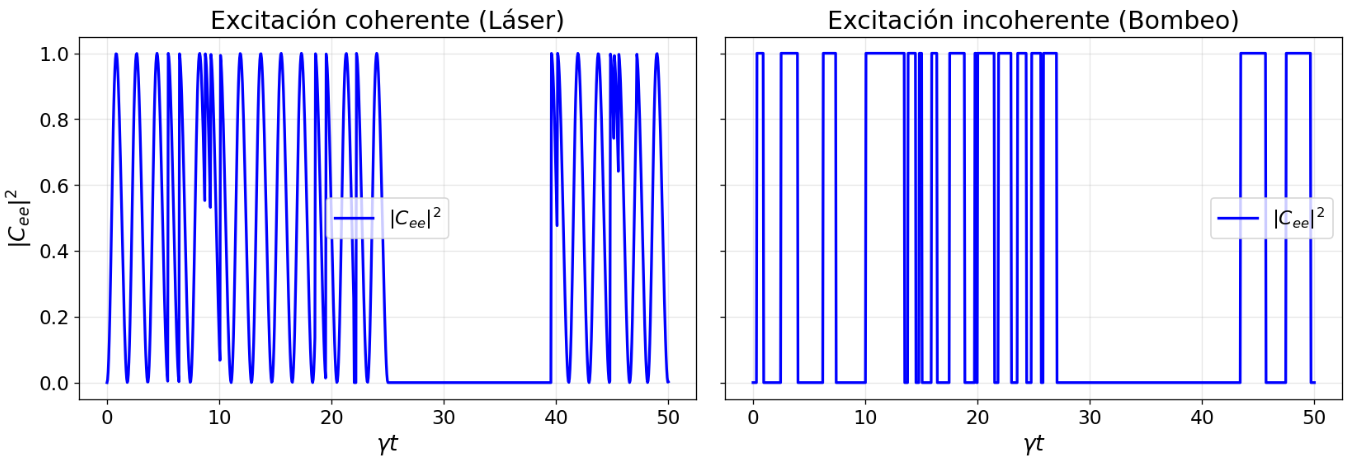
\includegraphics[width=0.9\textwidth]{imagenes/1tjinccoh.png}
    \caption{Comparación de una trayectoria individual de la población del estado excitado $\rho_{ee}(t) = |C_{ee}(t)|^2$ para excitación coherente (láser) e incoherente (bombeo). En el caso coherente se observan oscilaciones de Rabi y superposiciones, mientras que en el incoherente la dinámica es puramente estocástica con transiciones aleatorias entre los niveles.}
    \label{fig:comparacion_trayectorias_coh_incoh}
\end{figure}


\subsection{Convergencia de Trayectorias de Saltos}

El estado promedio de un sistema cuántico abierto puede obtenerse promediando un conjunto de $N$ realizaciones independientes de trayectorias de saltos cuánticos. En el límite termodinámico $N \to \infty$, el promedio de trayectorias converge a la solución de la ecuación maestra, de acuerdo con el teorema del límite central. El error estadístico de este promedio disminuye como $1/\sqrt{N}$, lo que implica que, al cuadruplicar el número de trayectorias, el error se reduce a la mitad.

Cada trayectoria cuántica representa una posible realización individual de un experimento. Debido a la naturaleza estocástica del método, una sola trayectoria contiene fluctuaciones intrínsecas y no coincide necesariamente con la solución promedio del sistema. Para reconstruir la dinámica física promedio, calculamos la matriz densidad promedio sumando $N$ trayectorias independientes. Conforme $N$ aumenta, el promedio estocástico se aproxima a la solución determinista de la ecuación maestra.

En la Figura~\ref{fig:convergencia_trayectorias} se muestra la población del estado excitado $\rho_{ee}(t)$ obtenida mediante el promedio de trayectorias de saltos para diferentes números de trayectorias, comparada con la solución exacta de la ecuación maestra (línea negra). Los valores de $N$ fueron elegidos de manera que cada caso tiene aproximadamente cuatro veces más trayectorias que el anterior: 157, 625, 2500 y 10000.

\begin{figure}[H]
    \centering
    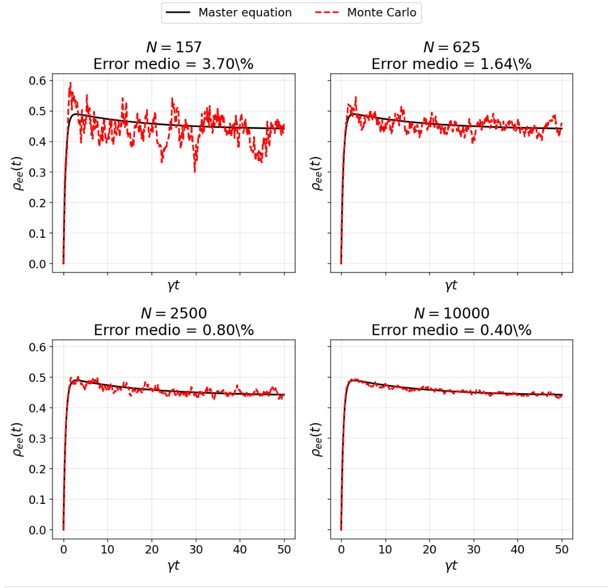
\includegraphics[width=0.9\textwidth]{imagenes/convergenciareal.png}
    \caption{Población del estado excitado $\rho_{ee}(t)$ obtenida mediante promedio de trayectorias de saltos para $N = 157, 625, 2500$ y $10000$ trayectorias (línea roja), comparada con la solución de la ecuación maestra (línea negra). El error disminuye como $1/\sqrt{N}$, visible en la reducción del ruido al aumentar $N$.}
    \label{fig:convergencia_trayectorias}
\end{figure}

Como se espera, el promedio de 10000 trayectorias reproduce prácticamente la solución de la ecuación maestra, con fluctuaciones despreciables. Para $N = 157$, en cambio, las desviaciones estadísticas son notables, reflejando el carácter estocástico del método. Se observa que al multiplicar $N$ por 4, el error se reduce aproximadamente por un factor de 2, consistente con el comportamiento predicho por el teorema del límite central. Este resultado valida la consistencia del método de trayectorias de saltos cuánticos y su capacidad para recuperar la dinámica promedio del sistema en el límite de muchas realizaciones.
\subsubsection{Distribución de Periodos Brillantes y Oscuros}

Finalmente, en la Figura~\ref{fig:distribucion_bombero_incoherente} se presentan las distribuciones de tiempos de los periodos brillantes y oscuros obtenidas a partir de simulaciones de trayectorias de saltos cuánticos para el átomo de tres niveles con bombeo incoherente. Los histogramas se comparan con las predicciones teóricas derivadas del modelo estocástico, donde los tiempos promedio están dados por

\begin{subequations}
\begin{eqnarray}
T_B &=& \frac{2\kappa + \gamma}{2\kappa \gamma_d}, \\
T_D &=& \gamma_a^{-1}.
\end{eqnarray}
\end{subequations}

De acuerdo con el modelo, tanto $P_B(t)$ como $P_D(t)$ siguen distribuciones exponenciales,

\begin{equation}
P_B(t) = T_B^{-1} e^{-t/T_B}, \qquad P_D(t) = T_D^{-1} e^{-t/T_D},
\end{equation}

lo que refleja la naturaleza markoviana de los procesos de conmutación entre periodos brillantes y oscuros.

\begin{figure}[H]
    \centering
    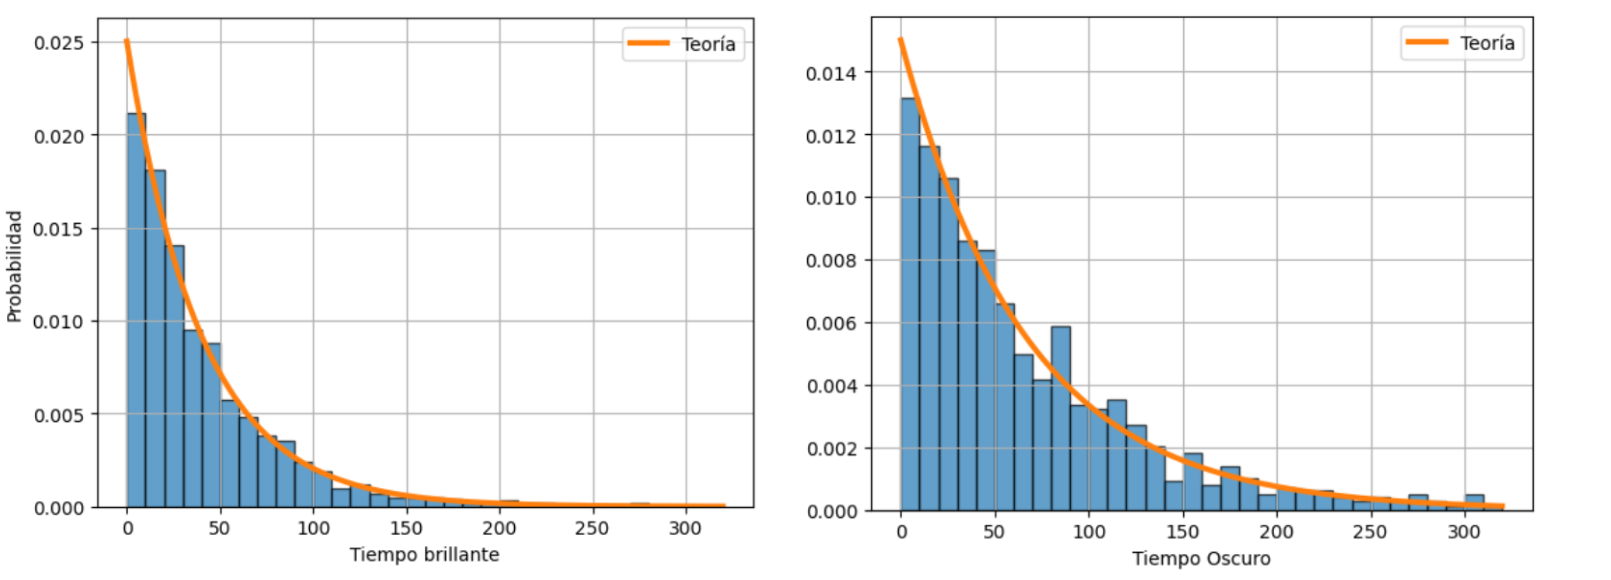
\includegraphics[width=0.8\textwidth]{imagenes/distTOTB.png}
    \caption{Distribuciones de tiempos de periodos brillantes $P_B(t)$ y oscuros $P_D(t)$ obtenidas de simulaciones de trayectorias de saltos cuánticos para el átomo de tres niveles con bombeo incoherente, comparadas con las predicciones teóricas exponenciales.}
    \label{fig:distribucion_bombero_incoherente}
\end{figure}

Los histogramas obtenidos numéricamente muestran un excelente acuerdo con las predicciones teóricas, validando así la consistencia del modelo estocástico para describir la dinámica de conmutación en el régimen de bombeo incoherente.
%Trabajo Futuro

\subsection{Reconstrucción del Espectro Completo: Suma de Cuadraturas}

Finalmente, en la Figura~\ref{fig:suma_cuadraturas_mollow} se presenta la suma de los espectros obtenidos en las cuadraturas $\theta = 0$ y $\theta = \pi/2$ mediante detección homodina balanceada. Como se ha mostrado, cada cuadratura captura una parte diferente del espectro de fluorescencia: la cuadratura $\theta = 0$ contiene el pico central coherente, mientras que la cuadratura $\theta = \pi/2$ revela los picos laterales inelásticos junto con el pico angosto asociado al shelving.

Al sumar ambas contribuciones, se obtiene el espectro completo de fluorescencia, el cual reproduce la estructura característica del triplete de Mollow. Este resultado demuestra que la combinación de las dos cuadraturas de la detección homodina permite reconstruir la totalidad del espectro, incluyendo tanto la componente elástica coherente como las componentes inelásticas laterales y la estructura fina introducida por el estado metaestable.

\begin{figure}[H]
    \centering
    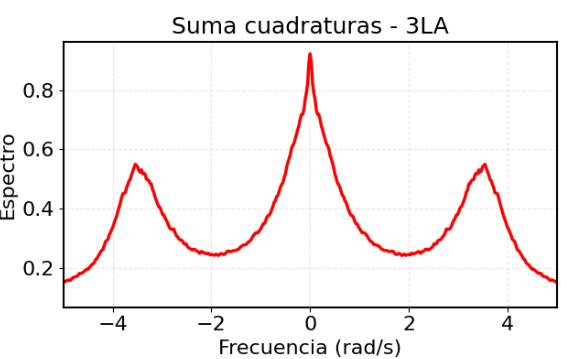
\includegraphics[width=0.9\textwidth]{imagenes/sumacuadraturas.png}
    \caption{Reconstrucción del espectro completo de fluorescencia mediante la suma de las cuadraturas $\theta = 0$ y $\theta = \pi/2$ de la detección homodina balanceada. La suma reproduce el triplete de Mollow característico de la fluorescencia resonante en un sistema de tres niveles.}
    \label{fig:suma_cuadraturas_mollow}
\end{figure}


\section{Perspectiva del Quinto Semestre}

Durante el presente semestre, realicé aportes sustanciales a ambos proyectos de investigación. Si bien los artículos correspondientes aún no están finalizados, se prevé que sean publicados antes de que concluya el año.

En el quinto semestre, se llevará a cabo la defensa de la tesis y se continuará contribuyendo al desarrollo de dos artículos de investigación en sistemas cuánticos abiertos, donde pueden aplicarse las ecuaciones de Schrödinger estocásticas. Las líneas de trabajo son las siguientes:

\begin{enumerate}
\item \textbf{Revisión, redacción y defensa de tesis.}

\item \textbf{Colaboración en estudios de radiación cooperativa.}
Se seguirá aportando a este proyecto como una línea de trabajo paralela a la tesis principal, con el objetivo de publicar un artículo. En particular, se continuará con el estudio teórico y numérico de sistemas compuestos por dos átomos en interacción, donde pueden emerger fenómenos de \textit{subradiancia} y \textit{superradiancia}. En dichos sistemas, simularé espectros dependientes del tiempo del tipo Eberly–Wódkiewicz variando parámetros tanto paramétricos como espaciales, con el fin de identificar comportamientos físicamente relevantes.

\item \textbf{Colaboración en estudios de bombeo incoherente en un átomo de tres niveles con \textit{shelving}}. con el objetivo de contribuir a la publicación de un artículo científico. Mi participación se centrará tanto en el análisis teórico mediante ecuaciones maestras como en la aplicación de ecuaciones de Schrödinger estocásticas. Inicialmente, el trabajo se enfocará en trayectorias cuánticas discontinuas y, posteriormente, si el tiempo y los objetivos del proyecto lo permiten, en trayectorias difusivas.
\end{enumerate}




\section{Cronograma de actividades}


\begin{table}[h!]
\centering
\renewcommand{\arraystretch}{1.5}
\begin{tabular}{|p{9cm}|c|c|c|c|c|}
\hline
\textbf{Actividad} & \multicolumn{5}{c|}{\textbf{Semestre}} \\ \cline{2-6} 
 & 1 & 2 & 3 & 4 & 5 \\ \hline

Búsqueda de información y análisis del estado del Arte & \cellcolor{green} & & & & \\ \hline
Estudio detallado de ecuaciones maestras y teoría de trayectorias cuánticas & \cellcolor{green} & & & & \\ \hline
Definición del marco teórico y planteamiento del problema & \cellcolor{green} & & & & \\ \hline

Definición de la metodología de simulación numérica (trayectorias cuánticas) & & \cellcolor{green} & & & \\ \hline
Selección y adaptación de herramientas computacionales (QuTiP, Python) & & \cellcolor{green} & & & \\ \hline
Elaboración del diseño de simulación (condiciones iniciales, parámetros, algoritmos) & & \cellcolor{green} & & & \\ \hline
Programación de simulaciones de trayectorias cuánticas para sistemas simples & & \cellcolor{green} & & & \\ \hline
Simulación y ajuste de parámetros (ejecución y depuración de código) & & \cellcolor{green} & & & \\ \hline
Análisis preliminar de resultados de simulaciones & & \cellcolor{green} & & & \\ \hline

Comparación con experimentos previos y ecuaciones maestras & & & \cellcolor{green} & & \\ \hline
Validación y ajuste de modelos teóricos & & & \cellcolor{green} & & \\ \hline
Discusión de resultados, refinamiento de hipótesis & & & \cellcolor{green} & & \\ \hline

Redacción del informe de investigación (marco teórico, metodología, resultados) & & & \cellcolor{green} & \cellcolor{green} & \cellcolor{green} \\ \hline
Preparación de presentaciones para congresos o seminarios & & & & \cellcolor{green} & \cellcolor{green} \\ \hline
Defensa del proyecto & & & & \cellcolor{green} & \cellcolor{green} \\ \hline

\end{tabular}
\end{table}



\newpage

\printbibliography

\end{document}
